\chapter{Dataset analysis and preparation}\label{ch:data-ana}

As mentioned in \Cref{ch:intro}, the dataset used in this thesis is the Indoor Location \& Navigation from kaggle, which was part of a competition of Microsoft Research in 2021 \cite{IndoorLocationNavigation}.
The company ``\(XYZ^{10}\)''\footnote{Website of \(XYZ^{10}\): \url{https://dangwu.io}} recorded the data in shopping malls and was provided by Microsoft Research for this competition.
The competition's goal was to predict the indoor position of users' smartphones based on real-time sensor data and user trace data.
The prediction for this competition contains the floor and waypoint at a particular timestamp.
However, this thesis will not predict the floor and waypoint but the following \ac{bssid} a device may connect to based on the \ac{rssi} of the \acp{ap} and the trajectory of the user, as this prediction is more beneficial for the roaming process.
Therefore, the dataset will be analyzed to determine what parts of the data I use for the \ac{ml} model.

\section{Components of the dataset}\label{sec:data}
As noted in the kaggle notebook ``Indoor Navigation: Complete Data Understanding'' \cite{IndoorNavigationUnderstanding} the data consists of 3 parts:

\begin{itemize}
    \item a \texttt{train} folder with train path files, organized by site and floor.
    \item a \texttt{test} folder with test path files, organized by site and floor but without waypoint data.
    \item a \texttt{metadata} folder with floor metadata, organized by site and floor, which includes floor images, further information, and a geojson map.
\end{itemize}

The train folder contains 204 subfolders representing each shopping mall (site) where data was recorded.
In each folder of the 204 subfolders, there are at least one and at most twelve subfolders representing the site's floors; the median is five floors.
Overall, there are 26,925 files, each containing the movement of a person for a specific site and floor.
Per floor, there are between one and 284 files with a median of 14.
The floor F1 of the site \begin{CJK*}{UTF8}{gbsn}银泰城(城西店)\end{CJK*} (Yintai City (Chengxi Branch)) in the train folder of the competition, has the most files.

The submission files and the test folder will not be used for this thesis.
Instead, I will generate the test set out of the train data because the goal is not to predict the floor and site name for a specific timestamp but to predict the \ac{bssid} to which a device may connect next, which is an entirely different task.
Therefore, I will not analyze the content of the test and metadata folders in detail but will further focus on the content of the train folder.


\section{File structure}\label{sec:file-structure}

Each file in each floor folder is a \textbf{.txt} file.
The first contains the start time of the recording, the second site information \texttt{SiteID} as hash, \texttt{SiteName}, \texttt{FloorId} as hash, and \texttt{FloorName}.

\lstset{
    basicstyle=\scriptsize\ttfamily,
    breaklines=true,
    escapeinside={(*@}{@*)},
    numbers=left,
    numberstyle=\tiny\color{gray},
    stepnumber=1,
    breakatwhitespace=true,
    xleftmargin=2.5em,
}

\begin{lstlisting}[caption={A snippet from the dataset of the file 5daa9e38df065a00069beb79.txt of the floor F4},label={lst:dataset}]
    #   startTime:1571462193934
    #   SiteID:5d27099303f801723c32364d SiteName:(*@\begin{CJK*}{UTF8}{gbsn}银泰百货(庆春店)\end{CJK*}@*) FloorId:5d27099303f801723c323650 FloorName:4F
    1571462193944   TYPE_WAYPOINT   57.885998   69.501526
    1571462194071   TYPE_ACCELEROMETER  -0.95254517 0.7944031   8.928757    2
    1571462194071   TYPE_MAGNETIC_FIELD -25.65918   -4.4784546  -28.201294  3
    1571462194071   TYPE_GYROSCOPE  -0.22373962 -0.07733154 -0.16847229 3
    1571462194071   TYPE_ROTATION_VECTOR    0.04186145  -0.02101801 -0.72491926 3
    1571462194071   TYPE_MAGNETIC_FIELD_UNCALIBRATED    -4.8568726  10.406494   -387.44965  20.802307   14.884949   -359.24835  3
    1571462194071   TYPE_GYROSCOPE_UNCALIBRATED -0.22218323 -0.068359375    -0.1628418  0.0026245117    9.765625E-4 -7.6293945E-4   3
    1571462194071   TYPE_ACCELEROMETER_UNCALIBRATED -0.95254517 0.7944031   8.928757    0.0 0.0 0.0 3
    ...
    1571462194883   TYPE_WIFI   b06c4e327882fab58dfa93ea85ca373a54e887b5    9f967858afcbb907af6e5adef766c7e7b936ef07    -63 2462    1571462190744
    1571462194883   TYPE_WIFI   8204870beb9d02995dab3f08aad97af5eab723cc    0413b35df78fc865af15b4721d5aeb33ff57da45    -64 2447    1571462188686
    ...
    1571462194020   TYPE_BEACON 07efd69e3167537492f0ead89fb2779633b04949    b6589fc6ab0dc82cf12099d1c2d40ab994e8410c    76e907e391ad1856762f70538b0fd13111ba68cd      -57 -71 5.002991815535578   1b7e1594febd760b00f1a7984e470867616cee4e    1571462194020
    ...
    1571462195943   TYPE_WAYPOINT   59.72475    69.02152
    #   endTime:1571462195976
\end{lstlisting}

The last line contains the end time of the recording.
The central part of the data consists of the collected data. 
Each line contains a UNIX timestamp in milliseconds, followed by a data type and the data itself, all separated by a tabulator.
The GitHub repository of the competition \footnote{The repository for the Indoor Location Competition 2.0: \url{https://github.com/location-competition/indoor-location-competition-20}} shows that the data type in the second column followed by its data can be one of the following:

\setlist[enumerate]{label=T\arabic*}
\begin{enumerate}
    \item\label{type:acce} \texttt{TYPE\_ACCELEROMETER} with x, y and z acceleration and an accuracy value.
    \item\label{type:mag}  \texttt{TYPE\_MAGNETIC\_FIELD} with x, y and z magnetic field and an accuracy value.
    \item\label{type:gyro}  \texttt{TYPE\_GYROSCOPE} with x, y and z gyroscope and an accuracy value.
    \item\label{type:rot}  \texttt{TYPE\_ROTATION\_VECTOR} with x, y and z rotation vector and an accuracy value.
    \item\label{type:mag_u}  \texttt{TYPE\_MAGNETIC\_FIELD\_UNCALIBRATED} with x, y and z magnetic field and an accuracy value.
    \item\label{type:gyro_u}  \texttt{TYPE\_GYROSCOPE\_UNCALIBRATED} with x, y and z gyroscope and an accuracy value.
    \item\label{type:acce_u}  \texttt{TYPE\_ACCELEROMETER\_UNCALIBRATED} with x, y and z acceleration and an accuracy value.
    \item\label{type:wifi}  \texttt{TYPE\_WIFI} with \ac{ssid}, \ac{bssid}, \ac{rssi}, frequency, and last seen timestamp of the access point. The SSID and BSSID are hashed.
    \item\label{type:beacon}  \texttt{TYPE\_BEACON} with \ac{uuid}, \ac{MajorID}, \ac{MinorID}, \ac{TxPower}, \ac{rssi}, distance to the device measured by the beacon, \ac{mac} address and a timestamp as padding data. The MajorID and MinorID are hashed.
    \item\label{type:way}  \texttt{TYPE\_WAYPOINT} with x and y coordinates, the ground truth locations labeled by the surveyor.
\end{enumerate}

Each file contains a different amount of waypoints and sensor data.
Each file's first and last data type is a \texttt{TYPE\_WAYPOINT}.
Lines with types from \ref{type:acce} to \ref{type:acce_u} occur every 20 ms and are measured at the same time.
\texttt{TYPE\_WIFI} occurs about every 1800-2200 ms.
\texttt{TYPE\_WAYPOINT} data is not evenly distributed.
Presumably, the waypoint data recording is triggered by an exterior event, e.g., a button press. 
As seen in \Cref{lst:dataset}, the data are measured separately from each other, so there are no combinations of the data types.
Most importantly, there is no combination of \texttt{TYPE\_WAYPOINT} and \texttt{TYPE\_WIFI} data, which would be needed for the prediction.
The location provided by \texttt{TYPE\_WAYPOINT} may be necessary because not only the strength of the \acp{rssi} is important but also the trajectory of the user, which can be identified by the \texttt{TYPE\_WAYPOINT} data.
Furthermore, the \ac{rssi} values may be influenced by the environment, e.g., walls, which may result in a lower \ac{rssi} value.

A prediction of the following \ac{bssid} will only work per site due to the different \acp{ap}.
Still, the prediction could be difficult for a whole site because the \acp{ap} are different on each floor, which may result in many \acp{ap} for the prediction.
Because the mall's first floor in Yintai City (Chengxi Branch) has the most trajectory data, this thesis will concentrate on that site for better prediction.
To further know how much data there is for the model's input, \Cref{tab:data_summary} shows a more detailed analysis.

\begin{table}[h]
    \centering
    \caption{Overview of data for F1 of site Yintai City (Chengxi Branch)}
    \begin{tabular}{|l|l|}
    \hline
    \textbf{Information} & \textbf{Value} \\ \hline
    Total data points & 7,157,081 \\ \hline
    Average data points per file & 25,201 \\ \hline
    Number of waypoints & 2,027 \\ \hline
    Lines of each \ref{type:acce} to \ref{type:acce_u} data & 746,689 \\ \hline
    Lines of \ac{wifi} data & 1,862,044 \\ \hline
    Lines of beacon data & 66,187 \\ \hline
    Number of \acp{bssid} & 4,795 \\ \hline
    Number of \acp{ap} & 4,795 \\ \hline
    Number of \acp{ssid} & 1,421 \\ \hline
    \ac{rssi} range & -93 to -13 dBm \\ \hline
    \end{tabular}
\label{tab:data_summary}
\end{table}


\section{Prepare data for an ML model}\label{sec:prep-on-data-for-an-ml-model}

As seen in previous sections, a location for the time of \texttt{TYPE\_WIFI} data points is not provided, but in order to predict the following \ac{bssid} more precisely than only using the \ac{rssi} from the \texttt{TYPE\_WIFI}, a location is needed.
Furthermore, there is also unnecessary data for the prediction, such as \texttt{TYPE\_BEACON} data.
Using the dataset for a \ac{ml} training requires further data preparation.
Details are given in the following.
As seen in \Cref{tab:data_summary}, this floor has 2,027 waypoints and 1,862,044 lines of \ac{wifi} data. Multiple lines per timestamp exist because the devices gather data from all nearby \acp{ap} for each timestamp.
\Cref{fig:vis-wo-interpolated} shows the waypoints.

\begin{figure}[h!]
    \centering
    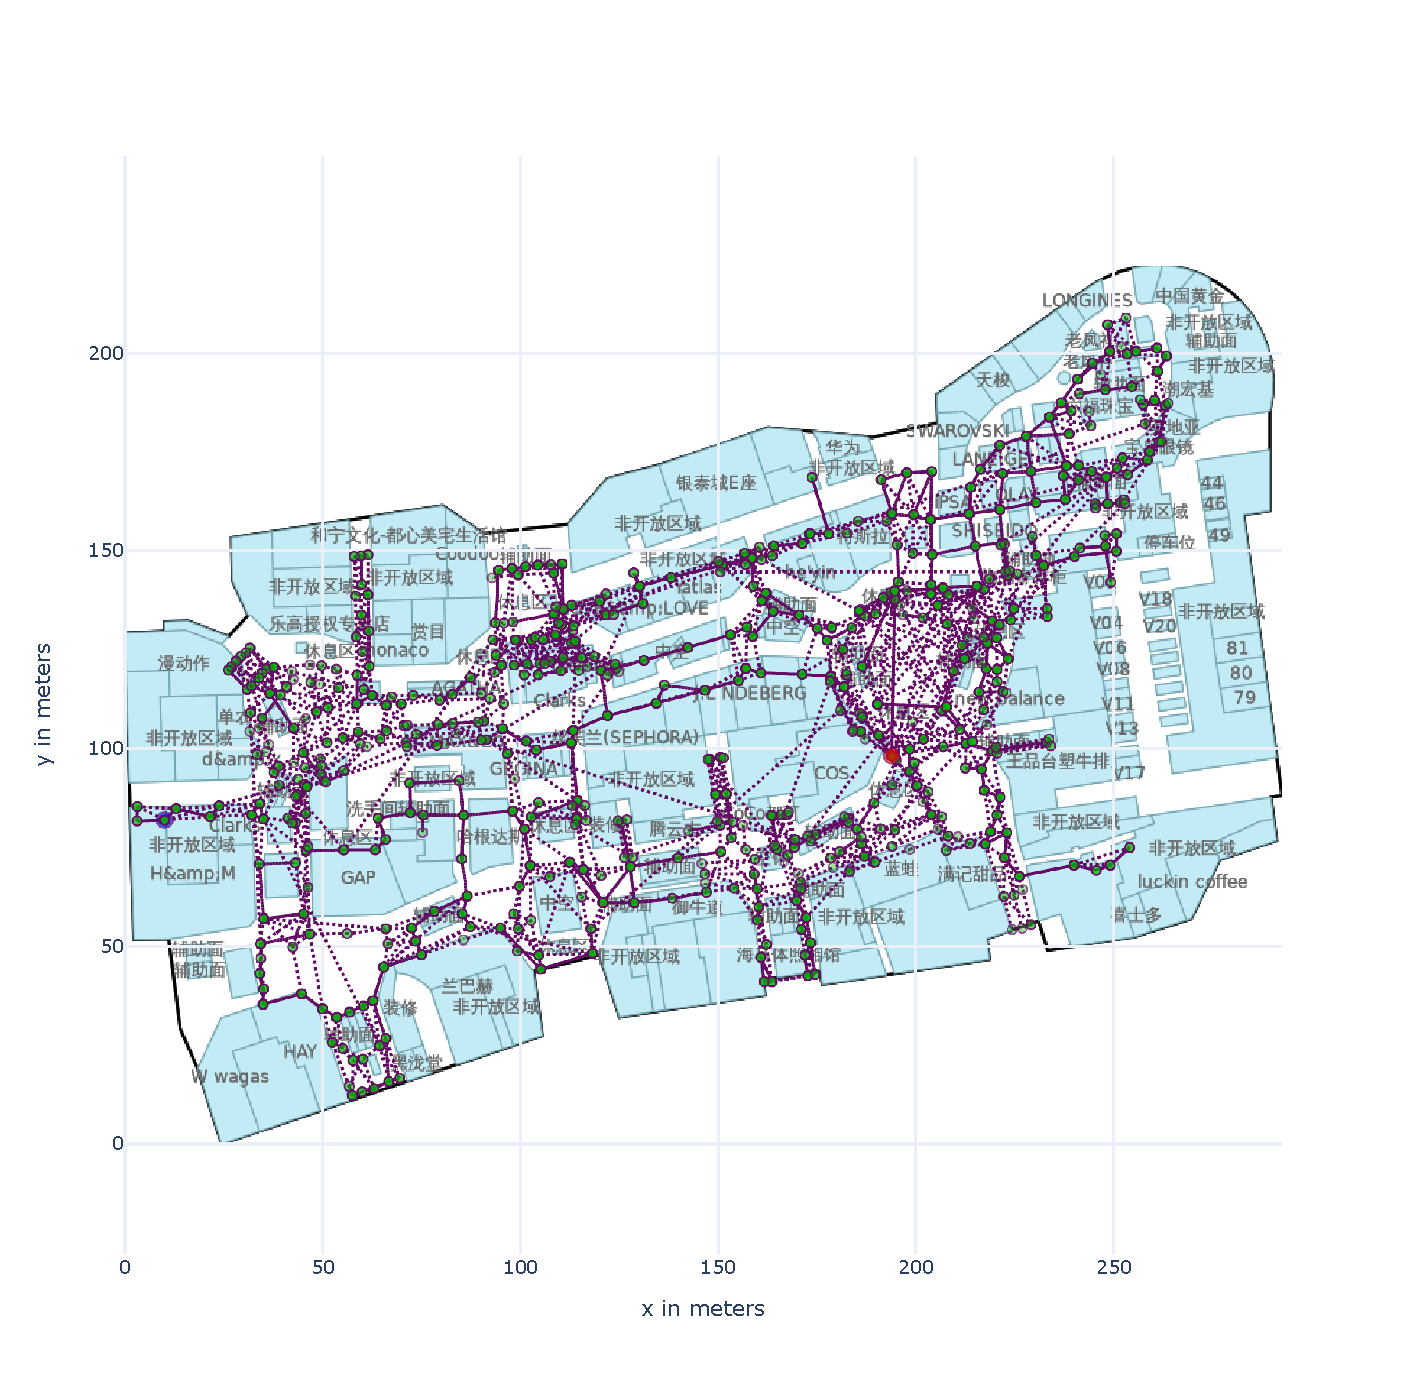
\includegraphics[scale=0.6]{images/whole_floor_visualization_wo_interpolated.pdf}
    \caption{Visualization of the 2,027 waypoints of the site Yintai City (Chengxi Branch) on floor F1}
    \label{fig:vis-wo-interpolated}
\end{figure}

Further human movement between \texttt{TYPE\_WAYPOINT} and \texttt{TYPE\_WIFI} data points may have occurred.
A concatenation of the data points to directly get the user's location for the \ac{wifi} data points will not work because the waypoint may have changed in that time or the \ac{rssi} value may have changed for the location.
Therefore, I choose to interpolate the data points of the \texttt{TYPE\_WAYPOINT} data for each \texttt{TYPE\_WIFI} timestamp.
%\fmhkn{I am still struggling why you even boterh with location??? is that really relevant? Why not just focus on RSSI, as stated above?}

Therefore, I perform an interpolation of \texttt{TYPE\_WAYPOINT} data for \texttt{TYPE\_WIFI} timestamps in order to get a location for the \ac{wifi}.
With this interpolation, a combination of \texttt{TYPE\_WAYPOINT} and \texttt{TYPE\_WIFI} data can be done, and more data could be used for the prediction.
The interpolation results in 6549 waypoints, three times more than the original waypoints, as seen in \Cref{fig:vis-interpolated}.

\begin{figure}[h!]
    \centering
    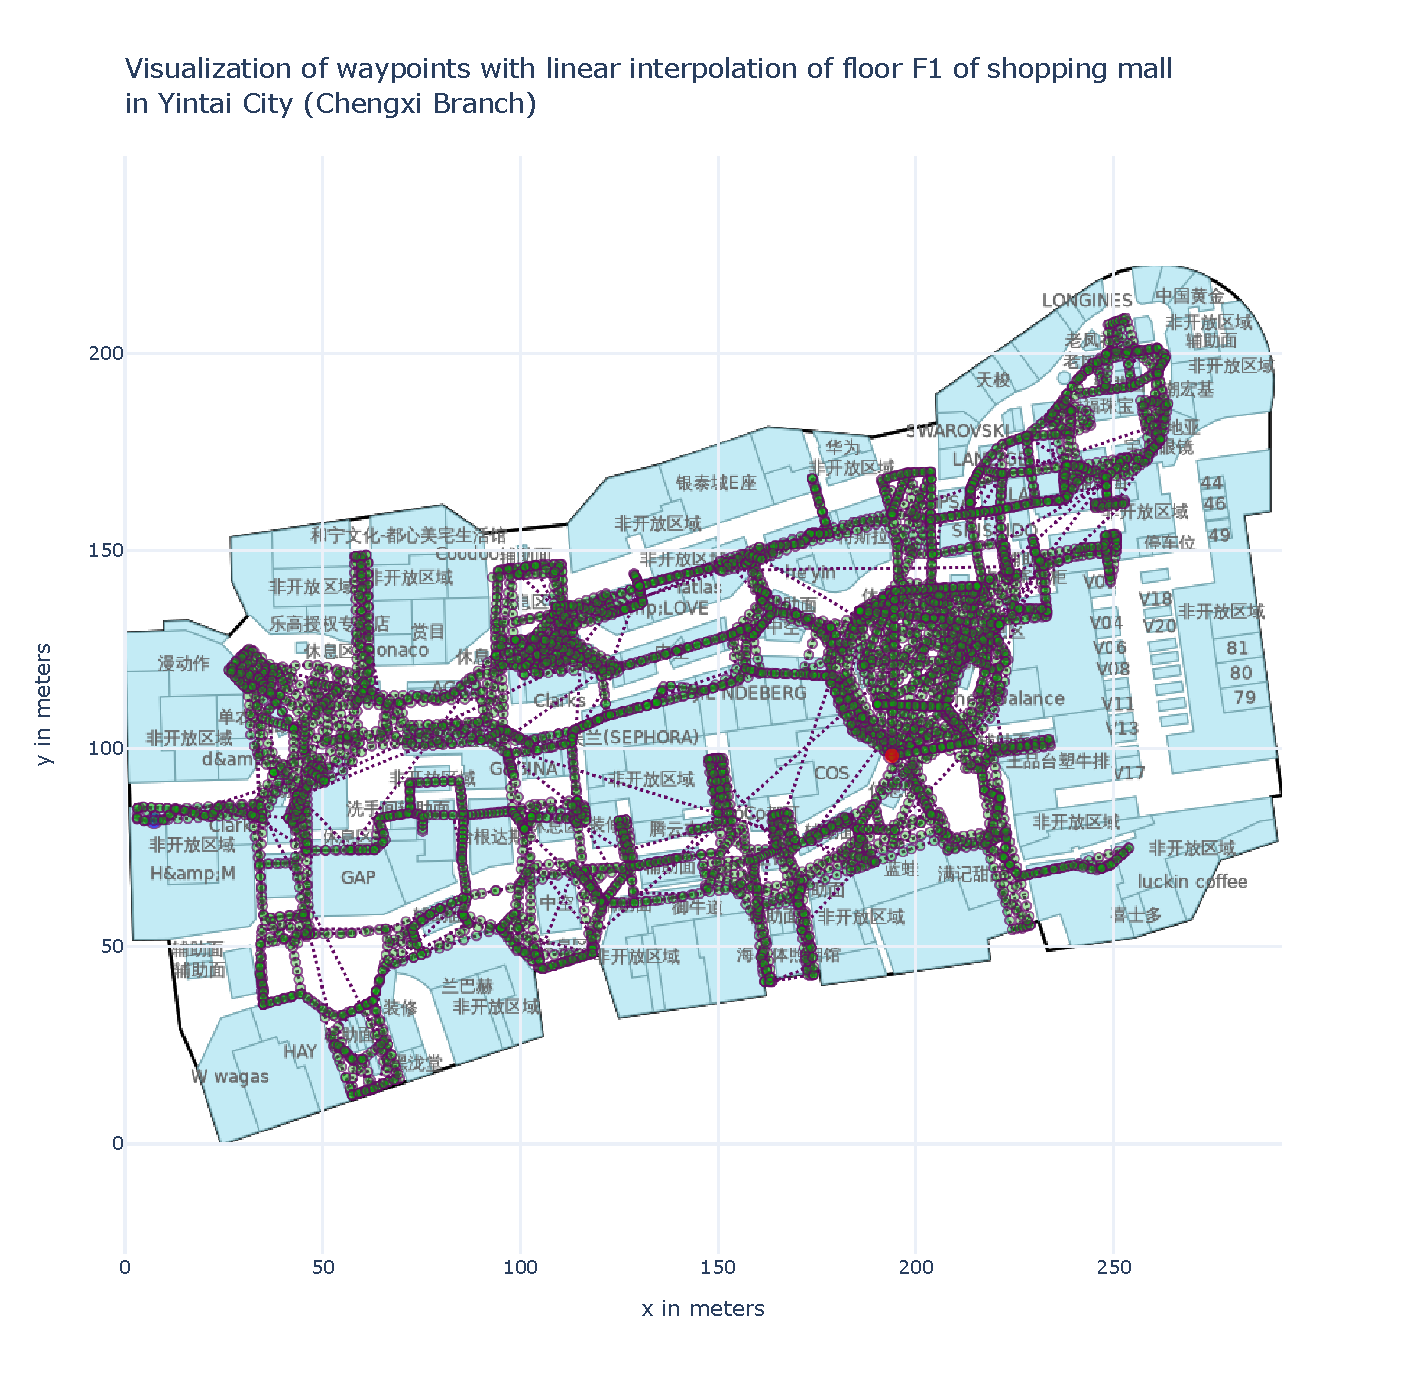
\includegraphics[scale=0.6]{images/whole_floor_visualization_interpolated.pdf}
    \caption{Visualization of the interpolated waypoints for site Yintai City (Chengxi Branch) on floor F1}
    \label{fig:vis-interpolated}
\end{figure}

As the \texttt{TYPE\_WAYPOINT} data may have changed, the \texttt{TYPE\_ACCELEROMETER} data may have changed as well.
Although the \texttt{TYPE\_ACCELEROMETER} data is measured every 20 ms, the \texttt{TYPE\_WIFI} data may not completely match the \texttt{TYPE\_ACCELEROMETER} timestamps.
Therefore, an interpolation of \texttt{TYPE\_ACCELEROMETER} data for \texttt{TYPE\_WIFI} timestamps is done.
The acceleration values may not change significantly, but it may result in a more accurate prediction than without interpolation.
A multivariate time series with \texttt{TYPE\_WAYPOINT} and \texttt{TYPE\_ACCELEROMETER} data for each \texttt{TYPE\_WIFI} timestamp is generated.
This time series will be used for the \ac{ml} model.
Further interpolation of the data, such as \texttt{TYPE\_GYROSCOPE}, is possible, but this thesis only utilizes the abovementioned data.


\subsection{Peculiarities of the data}\label{sec:special-cases}
The dataset analysis revealed some peculiarities, which are described in the following.

Different devices collect the data at different timestamps and days.
A problem for the time series is that the waypoint data were measured irregularly.
As \Cref{fig:vis-wo-interpolated} shows, some waypoints seem to be very distant from the next one, which can be detected by the dotted lines across the floor.
\Cref{tab:metric-diff} shows the top 10 pairs of waypoints with the most significant metric differences, where 174.77 meters is the most significant difference.

\begin{table}[h]
    \centering
    \caption{Top 10 pairs with the most significant metric differences of data from floor F1 of site Yintai City (Chengxi Branch)}
    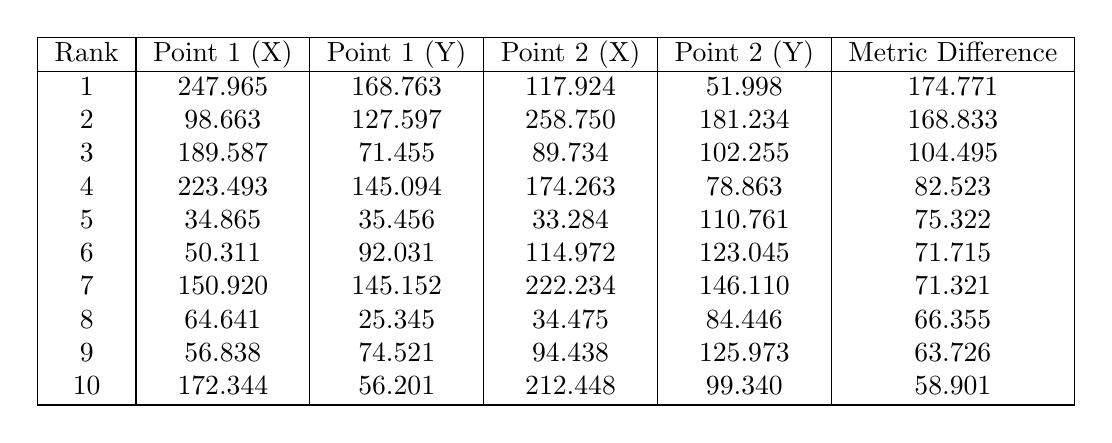
\begin{tikzpicture}
    \node (table) {
        \begin{tabular}{|c|c|c|c|c|c|}
        \hline
        Rank & Point 1 (X) & Point 1 (Y) & Point 2 (X) & Point 2 (Y) & Metric Difference \\
        \hline
        1 & 247.965 & 168.763 & 117.924 & 51.998 & 174.771 \\
        2 & 98.663 & 127.597 & 258.750 & 181.234 & 168.833 \\
        3 & 189.587 & 71.455 & 89.734 & 102.255 & 104.495 \\
        4 & 223.493 & 145.094 & 174.263 & 78.863 & 82.523 \\
        5 & 34.865 & 35.456 & 33.284 & 110.761 & 75.322 \\
        6 & 50.311 & 92.031 & 114.972 & 123.045 & 71.715 \\
        7 & 150.920 & 145.152 & 222.234 & 146.110 & 71.321 \\
        8 & 64.641 & 25.345 & 34.475 & 84.446 & 66.355 \\
        9 & 56.838 & 74.521 & 94.438 & 125.973 & 63.726 \\
        10 & 172.344 & 56.201 & 212.448 & 99.340 & 58.901 \\
        \hline
        \end{tabular}
    };
\end{tikzpicture}
    \label{tab:metric-diff}
\end{table}

This difference is too high for a human to walk in 1.8 to 2.2 seconds, the time between two waypoints.
A human's gait speed is maximum at about 2.53 meters per second \cite{bohannonComfortableMaximumWalking1997}.
So, in 2.2 seconds, a human can walk 5.57 meters, much less than each of the values in the top 10 in \Cref{tab:metric-diff}.
Therefore, waypoints that are more than 5.57 meters apart are defined as ``too apart from each other'' to walk in this time, and therefore, a split in the path will be done, and separated files will be generated, indicating a new path.
This results in 147 files with data interpolation, which will be used for the \ac{ml} model.
However, the data in those interpolated files does not contain any information about the \ac{bssid} and corresponding \ac{rssi} values, which are needed for the prediction.
This will be solved in the following \Cref{sec:wifi-data}.


\subsection{Wi-Fi data for each timestamp}\label{sec:wifi-data}
It is evident that for a waypoint, not all \ac{rssi} values for all \acp{ap} are present because the \ac{ap} may be out of range.
In order to use the \ac{rssi} in the prediction and treat each \ac{bssid} as a class for the \ac{ml} model, an \ac{rssi} value for each \ac{ap} for each timestamp is needed.

For this, all \acp{bssid} of the site will be gathered by iterating over all \ac{wifi} data and saved in one file.
Every line contains the timestamp, and each column header is the \ac{bssid} of the \ac{ap}, and each value of the line is the \ac{rssi} value of the \ac{bssid} at the timestamp.
If an \ac{ap} is absent, a very low value -999 is inserted because the typical \ac{rssi} value ranges from -55 to -90 \cite{rssi_calculation}.
This ensures that it is highly improbable for an \ac{ap} to be selected for the prediction with this value.
Then, I iterate over each file with interpolated data. For each timestamp, the \ac{bssid} and the corresponding \ac{rssi} value from the \ac{wifi} file are added to the interpolated file.
At each \texttt{TYPE\_WIFI} timestamp with waypoint and acceleration data, the \ac{rssi} value for each \ac{bssid} is now saved.

\section{Summary}
%\todo{include file structure and components}
The previous sections analyze the datasets and file structure.
The folder with the most user movement will be used for the prediction task.
The data was prepared into multivariate time series data for a \ac{ml} model based on \ac{wifi}, location, and acceleration data. 
An interpolation of the acceleration and waypoint data for each \texttt{TYPE\_WIFI} timestamp was necessary to combine this information for the prediction task.
The implementation of the preparation can be found in the GitHub repository \cite{github-repo} in the file ``preparation.ipynb''.
This prepared data will be further preprocessed in \Cref{ch:implementation} and utilized in the chosen \ac{ml} model, which will be discussed in the next Chapter.
